\chapter{Nginx}
\label{chap:nginx}

\section{关于Nginx}
\label{subsec:AboutNginx}

Nginx是由俄罗斯人Igor Sysoev为俄罗斯访问量第二Rambler.ru站
点开发的,它已经在该站点运行超过两年半了。它的发音为“engine
X”, 是一个高性能的HTTP和反向代理服务器,同时也是一个IMAP/POP3/SMTP 代
理服务器。Igor Sysoev在建立的项目时,使
用基于BSD许可。自Nginx发布四年来,Nginx已经因为它的稳定性、丰富的功能
集、示例配置文件和低系统资源的消耗而闻名。

在俄罗斯许多大网站都已经使用它,且一直表现不凡。截至2007年4月,俄罗斯
大约有20\%左右的虚拟主机是由Nignx服务或代理的。Google在线安全博客中统
计Nginx服务或代理了大约所有Internet虚拟主机的4\%。而Netcraft的统计显
示,Nginx服务的主机在过去的一年里以四倍的速度增长并且在这几年里,它的排
名还在不断上升,下图为Netcraft截止至2010年5月的统计。

\section{Nginx的安装与启动}
\label{subsec:InstallAndStartNginx}

Linux下安装软件有三种方式,这里我以源代码编译安装为主。服务器最小化安装
后,安装依赖包。

\begin{verbatim}
yum install -y pcre-devel \
gcc \
zlib-devel \
openssl-devel
\end{verbatim}

出于管理和安全的目的,我们希望使用一个指定的普通用户身份去运行我们的
Web服务器。所以,我们首先增加一个普通用户用于运行我们的Nginx。

\begin{verbatim}
groupadd nginx
useradd -g nginx nginx
\end{verbatim}

\begin{verbatim}
service iptables stop
chkconfig iptables off
\end{verbatim}

然后下载、解压并编译安装我们的Nginx,

\begin{verbatim}
wget http://nginx.org/download/nginx-1.8.0.tar.gz
tar -xf nginx-1.8.0.tar.gz -C /usr/local/src
cd /usr/local/src/nginx-1.8.0
./configure --user=nginx \
> --group=nginx \
> --with-http_ssl_module \
> --with-http_sub_module
\end{verbatim}

安装过程比较简单,./configure过程会报出一些依赖关系,这里已经解决。下面
来看看./configure后面几个常用的参数:

\begin{verbatim}
--prefix=<dir>         指定安装主目录,默认为/usr/local/nginx
--user=<user>          指定用户身份,如果没有指定则默认使用nobody
--group=<group>        指定组身份
--with-http_ssl_module 启用https支持
\end{verbatim}

\section{Nginx的基本配置}
\label{subsec:NginxConf}

Linux下基本上每个服务都会有它的主配置文件,该文件会定义服务应该如果去运
行,使用些什么参数,启用些什么功能,相关会涉及到的一些操作文件在哪,所
以主配置文件对服务是至关重要的。下面我们来分析一下Nginx的主配置文件。

\subsection{Nginx主配置概述}

Linux下基本上每个服务都会有它的主配置文件,该文件会定义服务应该如果去运
行,使用些什么参数,启用些什么功能,相关会涉及到的一些操作文件在哪,所以主
配置文件对服务是至关重要的。Nginx的主配置文件默认情况下位于
/usr/local/nginx/conf/nginx.conf,以下为Nginx配置文件一些参数的注释。

\begin{verbatim}
#user nobody;
#指定使用的用户
worker_processes 1;
#开启的进程数,一般设置 1-5
#error_log logs/error.log;
#error_log logs/error.log notice;
#error_log logs/error.log info;
#定义错误日志,以及记录的日志等级
#pid
logs/nginx.pid;
#定义 pid 文件位置
events {
# use [ kqueue | rtsig | epoll | /dev/poll | select | poll ];
#use epoll; #使用 epoll(linux2.6 的高性能方式)
#Nginx 支持如下处理连接的方法(I/O 复用方法),这些方法可以通过 use 指令指定。
#select - 标准方法。 如果当前平台没有更有效的方法,它是编译时默认的方法。你可以使用配置参
数 –with-select_module 和 –without-select_module 来启用或禁用这个模块。
#poll - 标准方法。 如果当前平台没有更有效的方法,它是编译时默认的方法。你可以使用配置参数
–with-poll_module 和 –without-poll_module 来启用或禁用这个模块。
#kqueue - 高效的方法,使用于 FreeBSD 4.1+, OpenBSD 2.9+, NetBSD 2.0 和 MacOS X. 使用双
处理器的 MacOS X 系统使用 kqueue 可能会造成内核崩溃。
#epoll - 高效的方法,使用于 Linux 内核 2.6 版本及以后的系统。在某些发行版本中,如 SuSE 8.2,
有让 2.4 版本的内核支持 epoll 的补丁。
#rtsig - 可执行的实时信号,使用于 Linux 内核版本 2.2.19 以后的系统。可是从 Linux 内核版本
2.6.6-mm2 开始,这个参数就不再使用了.
#/dev/poll - 高效的方法,使用于 Solaris 7 11/99+, HP/UX 11.22+ (eventport), IRIX 6.5.15+ 和
Tru64 UNIX 5.1A+.
#eventport - 高效的方法,使用于 Solaris 10. 为了防止出现内核崩溃的问题, 有必要安装这个安全补丁。
worker_connections 1024;
#worker_connections 51200; #每个进程最大连接数(最大连接=连接数 x 进程数)
}
http {
include
mime.types;
#文件扩展名与文件类型映射表
default_type application/octet-stream;
#默认文件类型
#log_format main '$remote_addr - $remote_user [$time_local] "$request" '
# '$status $body_bytes_sent "$http_referer" '
# '"$http_user_agent" "$http_x_forwarded_for"';
#access_log logs/access.log main;
sendfile
on;
#开启高效文件传输模式
#tcp_nopush
on;
#该选项用于防止网络阻塞
#keepalive_timeout 0;
keepalive_timeout 65;
##长链接超时时间
#gzip on;
#打开 gzip 压缩
#fastcgi_connect_timeout 300;
#fastcgi_send_timeout 300;
#fastcgi_read_timeout 300;
#fastcgi_buffer_size 128k;
#fastcgi_buffers 4 256k;
#fastcgi_busy_buffers_size 256k;
#fastcgi_temp_file_write_size 256k;
#fastcgi_temp_path /dev/shm;
#fastcgi 连接超时时间和缓存
server {
listen
80;
server_name localhost;
#主机名
#charset koi8-r;
#默认字符编码 charset gb2312
#access_log logs/host.access.log main;
location / {
#pass 路径匹配 能够匹配路径中带“/”的 不过需要注意的是如果之后也有相关“/”匹配项并且
使用比此处更精确匹配符,则以之后表达式优先
root html;
index index.html index.htm;
}
#error_page 404
/404.html;
# redirect server error pages to the static page /50x.html
#
error_page 500 502 503 504 /50x.html;
location = /50x.html {
#精确的匹配,并且不再向下匹配
root html;
}
#
#location ~ \.php$ {
#正则表达式匹配 一旦匹配则不再向下匹配
#
proxy_pass http://127.0.0.1;
#}
# pass the PHP scripts to FastCGI server listening on 127.0.0.1:9000
#
#location ~ \.php$ {
# root
html;
# fastcgi_pass 127.0.0.1:9000;
#指定 fastcgi 的地址端口
# fastcgi_index index.php;
# fastcgi_param SCRIPT_FILENAME /scripts$fastcgi_script_name;
# include fastcgi_params;
#}
# deny access to .htaccess files, if Apache's document root
# concurs with nginx's one
#
#location ~ /\.ht {
#
deny all;
#不允许访问以.ht 开头的文件
#}
}
# another virtual host using mix of IP-, name-, and port-based configuration
#
#server {
# listen
8000;
# listen
somename:8080;
# server_name somename alias another.alias;
# location / {
# root html;
# index index.html index.htm;
#
}
#}
#以上在配置虚拟主机
# HTTPS server
#
#server {
# listen 443;
# server_name localhost;
# ssl on;
# ssl_certificate cert.pem;
# ssl_certificate_key cert.key;
# ssl_session_timeout 5m;
# ssl_protocols SSLv2 SSLv3 TLSv1;
# ssl_ciphers ALL:!ADH:!EXPORT56:RC4+RSA:+HIGH:+MEDIUM:+LOW:+SSLv2:+EXP;
# ssl_prefer_server_ciphers on;

#以上为 ssl 配置
# location / {
# root html;
# index index.html index.htm;
# }
# }
}
\end{verbatim}

\subsection{Nginx虚拟主机配置}

利用虚拟主机技术,可以把一台真正的主机分成许多虚拟的主机,每一台虚拟主
机都具有独立的域名和IP地址,具有完整的Internet服务器(www,FTP,email)
功能。虚拟主机之间完全独立,在外界看来,每一台虚拟主机和一台独立的主机
完全一样。效果一样但费用却大不一样了。由于多台虚拟主机共享一台真实主机
的资源,每个虚拟主机用户承受的硬件费用、网络维护费用、通信线路的费用均
大幅度降低,Internet真正成为人人用得起的网络!

虚拟主机共分为三种:基于IP的虚拟主机,基于端口的虚拟主机和基于名称的虚拟
主机。前两种由于受到成本和客户使用习惯的限制,相对使用的没有基于名称的
虚拟主机多,以下我们介绍一下三种虚拟主机的配置。

\subsection{安全的连接https}

众所周知,我们在互联网上冲浪,一般使用的是http协议(超文本传输协议),
默认情况下数据是明文传送的,这些数据在传输过程中都可能会被捕获和窃听,
因此是不安全的。https可以说是http协议的安全版,就是为了满足对安全性要求
比较高的用户而设计的。

\section{Nginx日志管理}

\section{Nginx访问控制}

\section{Nginx反向代理}
\label{subsec:NginxReverseProxy}

反向代理(Reverse Proxy)方式是指以代理服务器来接受Internet上的连接请求,
然后将请求转发给内部网络上的服务器,并将从服务器上得到的结果返回
给Internet上请求连接的 客户端,此时代理服务器对外就表现为一个服务器。

反向代理又称为Web服务器加速,是针对Web服务器提供加速功能的。它作为代
理Cache,但并不针对浏览器用户,而针对一台或多台特定Web服务器(这也是反
向代理名称的由来)。代理服务器可以缓存一些web的页面,降低了web服务器的
访问量,所以可以降低web服务器的负载。web服务器同时处理的请求数少了,响
应时间自然就快了。同时代理服务器也存了一些页面,可以直接返回给客户端,
加速客户端浏览。实施反向代理,只要将反向代理设备放置在一台或多台Web服务
器前端即可。当互联网用户访问某个WEB服务器时,通过DNS服务器解析后的IP地
址是代理服务器的IP地址,而非原始Web服务器的IP地址,这时代理服务器设备充
当Web服务器,浏览器可以与它连接,无需再直接与Web服务器相连。因此,大
量Web服务工作量被转载到反向代理服务上。不但能够很大程度上减轻web服务器
的负担,提高访问速度,而且能够防止外部网主机直接和web服务器直接通信带来
的安全隐患。

\begin{figure}[!h]
  \centering
  \subfloat[squid代理模式]{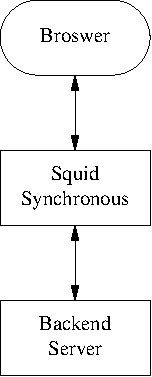
\includegraphics[width=.2\textwidth]{graph/reverse_squid.pdf}}\hspace{30pt}
  \subfloat[nginx代理模式]{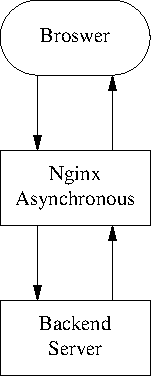
\includegraphics[width=.2\textwidth]{graph/reverse_nginx.pdf}}
  \caption{两种代理模式比较}
  \label{fig:squidVSnginx}
\end{figure}

squid同步传输:浏览器发起请求,而后请求会立刻被转到后台,于是在浏览器和
后台之间就建立了一个通道。在请求发起直到请求完成,这条通道都是一直存在
的。

nginx异步传输:浏览器发起请求,请求不会立刻转到后台,而是将请求数据(
header )先收到nginx上,然后nginx再把这个请求发到后端, 后端处理完之后把数
据返回到nginx上, nginx将数据流发到浏览器,这点和lighttpd有点不同,
lighttpd是将后端数据完全接收后才发送到浏览器。

那么这到底有什么好处呢?

\begin{enumerate}[itemsep=0pt,parsep=0pt]
\item 假设用户执行一个上传文件操作,因为用户网速又比较慢,因此需要花半
  个小时才能把文件传到服务器。squid的同步代理在用户开始上传后就和后台建
  立了连接,半小时后文件上传结束,由此可见,后台服务器连接保持了半个小
  时;而 nginx异步代理就是先将此文件收到nginx上,因此仅仅是nginx和用户
  保持了半小时连接,后台服务器在这半小时内没有为这个请求开启连接,半小
  时后用户上传结束,nginx才将上传内容发到后台,nginx和后台之间的带宽是
  很充裕的,所以只花了一秒钟就将请求发送到了后台,由此可见,后台服务器
  连接保持了一秒。同步传输花了后台服务器半个小时,异步传输只花一秒,可
  见优化程度很大。

\item 在上面这个例子中,假如后台服务器因为种种原因重启了,上传文件就自
  然中断了,这对用户来说是非常恼火的一件事情,想必我们也有上传文件传到
  一半被中断的经历。用nginx代理之后,后台服务器的重启对用户上传的影响减
  少到了极点,而nginx是非常稳定的并不需要常去重启它,即使需要重启,利用
  kill -HUP就可以做到不间断重启nginx。

\item 异步传输可以令负载均衡器更有保障,为什么这么说呢?在其它的均衡器
  ( lvs/haproxy/apache 等)里,每个请求都是只有一次机会的,假如用户发起
  一个请求,结果该请求分到的后台服务器刚好挂掉了,那么这个请求就失败了;
  而 nginx因为是异步的,所以这个请求可以重新发往下一个后台,下一个后台
  返回了正常的数据,于是这个请求就能成功了。还是用用户上传文件这个例子,
  假如不但用了nginx代理,而且用了负载均衡,nginx把上传文件发往其中一台
  后台,但这台服务器突然重启了,nginx收到错误后,会将这个上传文件发到另
  一台后台,于是用户就不用再花半小时上传一遍。

\item 假如用户上传一个10GB大小的文件,而后台服务器没有考虑到这个情况,
  那么后台服务器岂不要崩溃了。用nginx就可以把这些东西都拦在nginx上, 通
  过nginx的上传文件大小限制功能来限制,另外nginx性能非常有保障,就放心
  的让互联网上那些另类的用户和nginx对抗去吧。
\end{enumerate}

\subsection{Nginx 与 Lua 结合}

%%% Local Variables:
%%% mode: latex
%%% TeX-master: t
%%% End:
